% ----------------------------------------------------------
% ESTATÍSTICA DOS REPOSITÓRIOS
% ----------------------------------------------------------
\section{Estatísticas dos repositórios}
Nesta seção serão apresentadas as estatísticas de cada versionador de código, com detalhes da atuação de cada integrante da equipe e dos commits feitos durante o desenvolvimento.

\subsection{SVN}
Estatísticas sobre o repositório no \gls{svn} foram geradas através do \gls{statsvn} apesar de não ter sido usado como nosso versionador principal, então os dados sobre os autores que participaram não devem ser considerados como a realidade. Usamos o SVN por ser obrigatório no projeto e fizemos atualizações esporádicas lá com nosso código versionado no Git.

A \autoref{svn-lines-code} mostra a evolução de linhas de código conforme o tempo.
\begin{figure}[H]
	\centering
	\caption{\label{svn-lines-code}Linhas de código - SVN}
	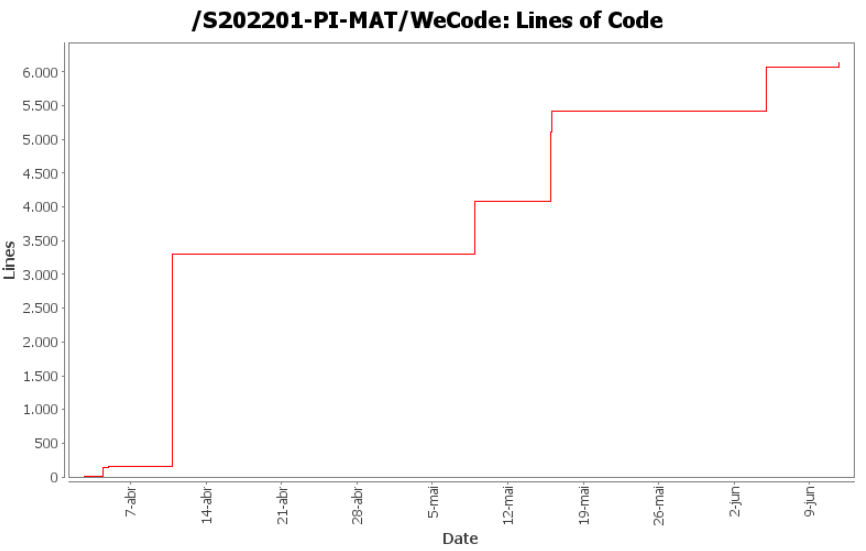
\includegraphics[width=0.95\textwidth]{../imagens/stats/svn-lines-code.png}
	\fonte{Os autores - Criado via \gls{statsvn}}
\end{figure}

A \autoref{svn-author-activity} mostra as atividades dos autores participantes no repositório. Cabendo ressaltar que não condiz com a realidade.
\begin{figure}[H]
	\centering
	\caption{\label{svn-author-activity}Atividade dos autores - SVN}
	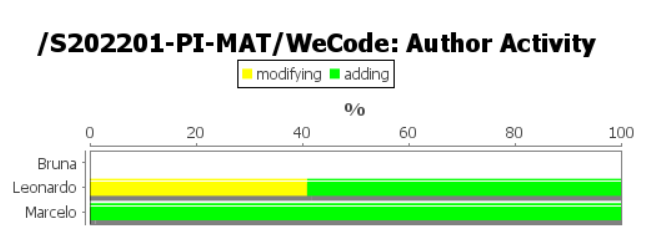
\includegraphics[width=0.95\textwidth]{../imagens/stats/svn-author-activity.png}
	\fonte{Os autores - Criado via \gls{statsvn}}
\end{figure}

A \autoref{svn-activity-day} mostra a quantidade de commits por dia da semana.
\begin{figure}[H]
	\centering
	\caption{\label{svn-activity-day}Atividade por dia da semana - SVN}
	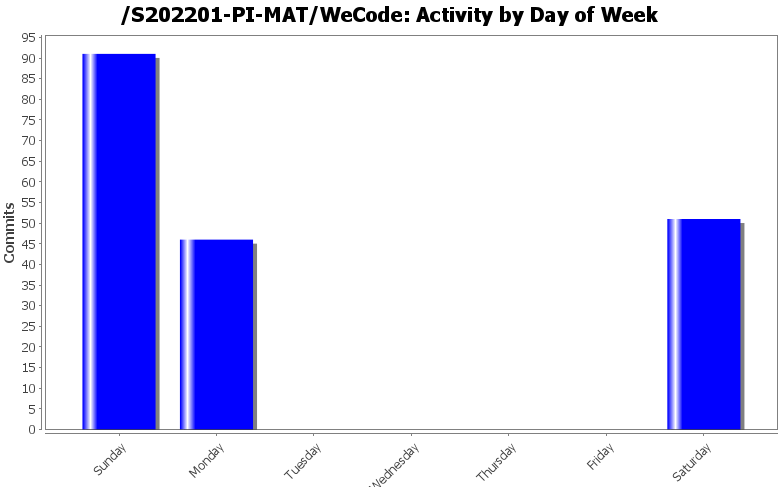
\includegraphics[width=0.95\textwidth]{../imagens/stats/svn-activity-day.png}
	\fonte{Os autores - Criado via \gls{statsvn}}
\end{figure}

\subsection{GitHub}
A partir dos commits feitos nos repositórios, levantamos estatísticas sobre nosso projeto através do \gls{gitstats}, que servem de base para termos uma ideia de como foi o andamento do projeto e o que cada integrante da equipe fez durante o período.
O \gls{git} foi usado como nosso versionador principal, então os dados abaixo estão bem próximos da realidade.

A \autoref{overview-front} demonstra uma visão geral sobre alguns dados do repositório onde hospedamos o nosso \gls{frontend}.
\begin{pspicture}(25mm,25mm)
    \psbarcode{https://github.com/EquipeWeCode/estagiei-frontend}{eclevel=H width=1.0 height=1.0}{qrcode}
\end{pspicture}
\begin{figure}[H]
	\centering
	\caption{\label{overview-front}Visão geral - Projeto \gls{frontend}}
	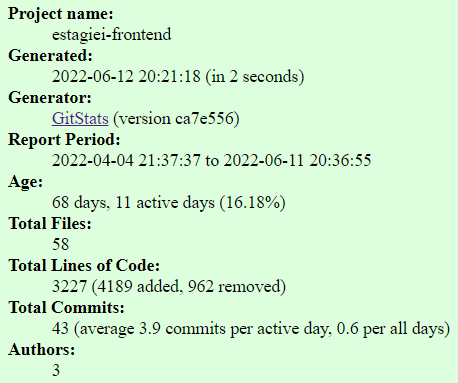
\includegraphics[width=0.95\textwidth]{../imagens/stats/overview-frontend.png}
	\fonte{Os autores - Criado via \gls{gitstats}}
\end{figure}

A \autoref{overview-back} demonstra uma visão geral sobre alguns dados do repositório onde hospedamos o nosso backend, e podemos notar algumas diferenças entre ele e o \gls{frontend}.

\begin{pspicture}(25mm,25mm)
    \psbarcode{https://github.com/EquipeWeCode/estagiei-backend}{eclevel=H width=1.0 height=1.0}{qrcode}
\end{pspicture}

\begin{figure}[H]
	\centering
	\caption{\label{overview-back}Visão geral - Projeto Backend}
	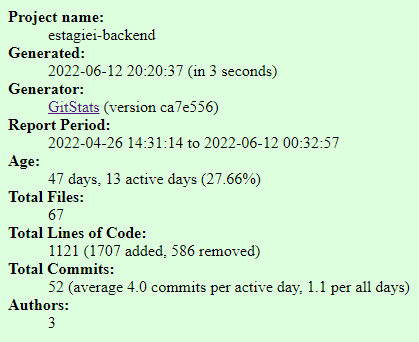
\includegraphics[width=0.95\textwidth]{../imagens/stats/overview-backend.png}
	\fonte{Os autores - Criado via \gls{gitstats}}
\end{figure}

A \autoref{overview-doc} demonstra uma visão geral sobre alguns dados principais do nosso repositório onde versionamos os documentos latex do nosso projeto.

\begin{pspicture}(25mm,25mm)
    \psbarcode{https://github.com/EquipeWeCode/documentos}{eclevel=H width=1.0 height=1.0}{qrcode}
\end{pspicture}

\begin{figure}[H]
	\centering
	\caption{\label{overview-doc}Visão geral - Projeto Documentos}
	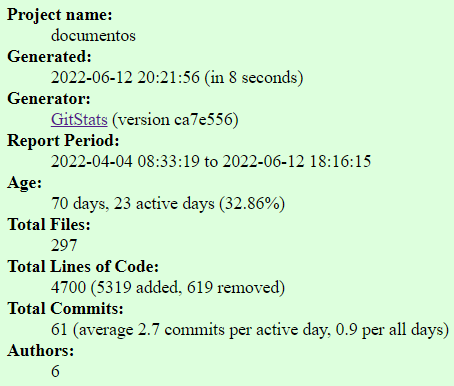
\includegraphics[width=0.95\textwidth]{../imagens/stats/overview-documentos.png}
	\fonte{Os autores - Criado via \gls{gitstats}}
\end{figure}

A \autoref{lines-of-code-front} demonstra a evolução em número de linhas do nosso repositório do projeto \gls{frontend}.
\begin{figure}[H]
	\centering
	\caption{\label{lines-of-code-front}Linhas de código - Projeto \gls{frontend}}
	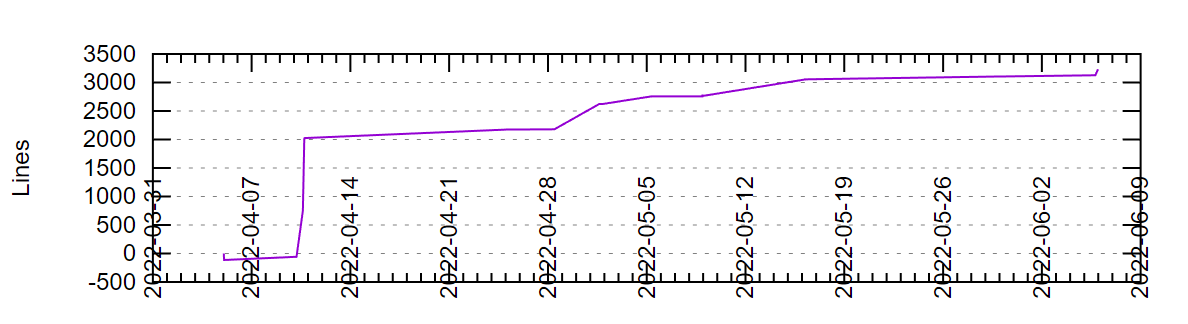
\includegraphics[width=0.95\textwidth]{../imagens/stats/lines-of-code-frontend.png}
	\fonte{Os autores - Criado via \gls{gitstats}}
\end{figure}

A \autoref{lines-of-code-back} demonstra a evolução em número de linhas do nosso repositório do projeto backend.
\begin{figure}[H]
	\centering
	\caption{\label{lines-of-code-back}Linhas de código - Projeto Backend}
	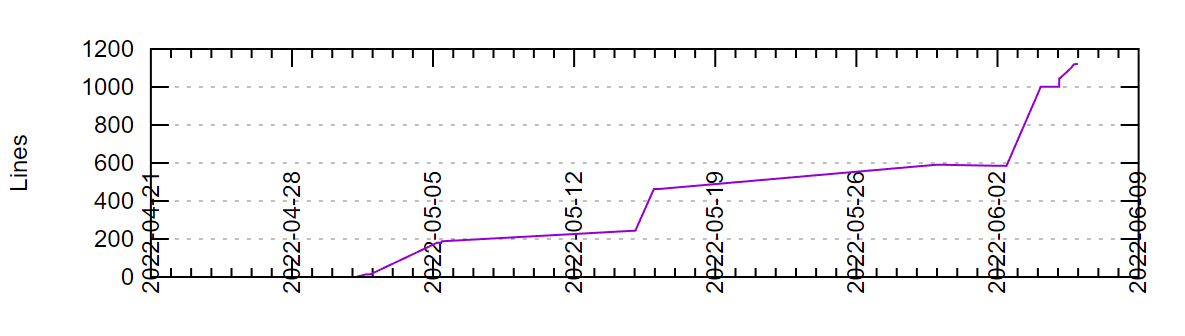
\includegraphics[width=0.95\textwidth]{../imagens/stats/lines-of-code-backend.png}
	\fonte{Os autores - Criado via \gls{gitstats}}
\end{figure}

Cabe ressaltar que o número de linhas não necessariamente diz que criamos muito código, como demonstra a \autoref{extensions-frontend}, grande parte das linhas do nosso \gls{frontend} são de arquivos .json, principalmente do package-lock.json, que é gerado automaticamente e documenta e versiona as dependências do nosso projeto.
\begin{figure}[H]
	\centering
	\caption{\label{extensions-frontend}Extensão de arquivos - Projeto \gls{frontend}}
	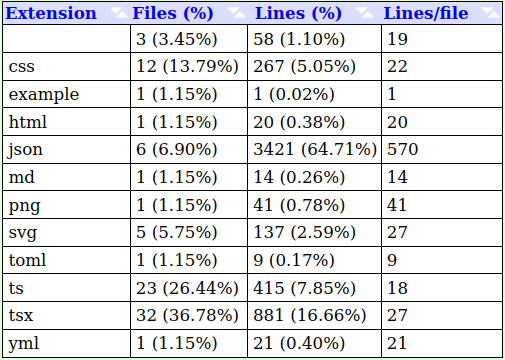
\includegraphics[width=0.95\textwidth]{../imagens/stats/extensions-frontend.png}
	\fonte{Os autores - Criado via \gls{gitstats}}
\end{figure}

A \autoref{list-of-authors-front} lista os autores que contribuíram no repositório \gls{frontend}. Cabe ressaltar que o autor Leonardo Marques e o LeonMarqs são a mesma pessoa, que por algum motivo ficaram separadas nas estatísticas.
\begin{figure}[H]
	\centering
	\caption{\label{list-of-authors-front}Dias da semana - Projeto \gls{frontend}}
	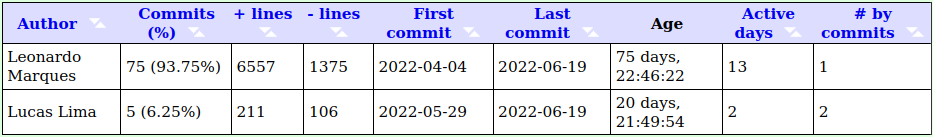
\includegraphics[width=0.95\textwidth]{../imagens/stats/list-of-authors-frontend.png}
	\fonte{Os autores - Criado via \gls{gitstats}}
\end{figure}

A \autoref{list-of-authors-back} lista os autores que contribuíram no repositório backend.
\begin{figure}[H]
	\centering
	\caption{\label{list-of-authors-back}Lista de autores - Projeto Backend}
	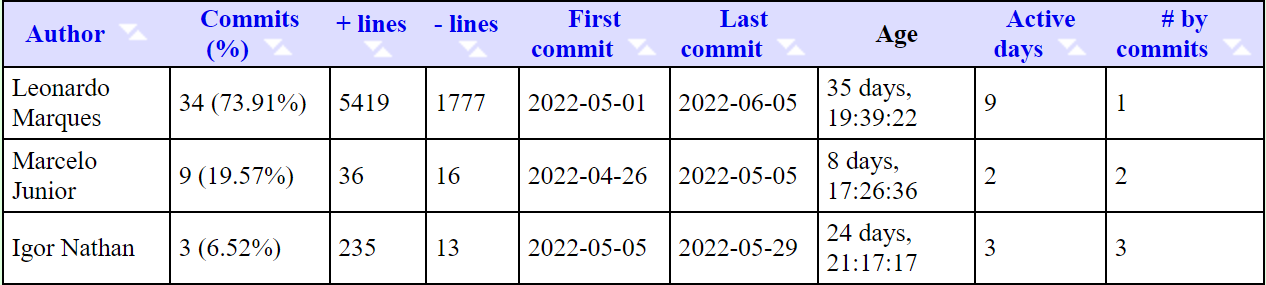
\includegraphics[width=0.95\textwidth]{../imagens/stats/list-of-authors-backend.png}
	\fonte{Os autores - Criado via \gls{gitstats}}
\end{figure}

A \autoref{list-of-authors-doc} lista os autores que contribuíram no repositório de documentos, onde houve o mesmo problema de separação da mesma pessoa (Leonardo Marques).
\begin{figure}[H]
	\centering
	\caption{\label{list-of-authors-doc}Lista de autores - Projeto Documentos}
	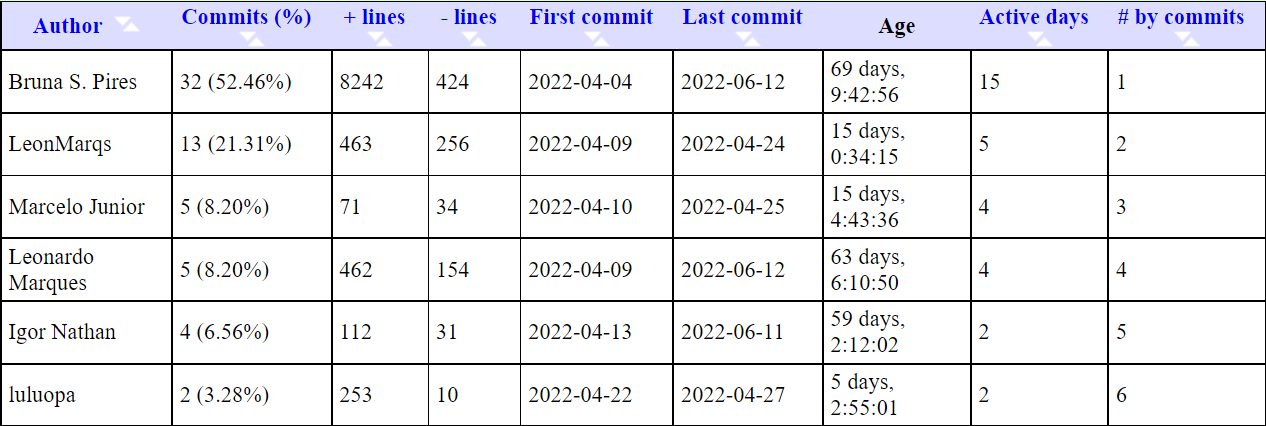
\includegraphics[width=0.95\textwidth]{../imagens/stats/list-of-authors-documentos.png}
	\fonte{Os autores - Criado via \gls{gitstats}}
\end{figure}

A \autoref{days-of-week-frontend} mostra os dias da semana em que foram feitos mais commits no repositório \gls{frontend}. (Sendo 1 = segunda).
\begin{figure}[H]
	\centering
	\caption{\label{days-of-week-frontend}Dias da semana - Projeto \gls{frontend}}
	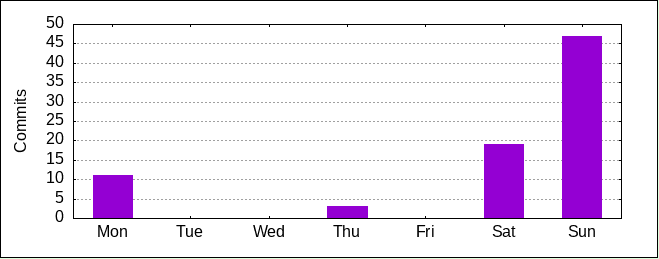
\includegraphics[width=0.95\textwidth]{../imagens/stats/days-of-week-frontend.png}
	\fonte{Os autores - Criado via \gls{gitstats}}
\end{figure}

A \autoref{days-of-week-frontend} mostra os dias da semana em que foram feitos mais commits no repositório backend. (Sendo 1 = segunda).
\begin{figure}[H]
	\centering
	\caption{\label{days-of-week-backend}Dias da semana - Projeto Backend}
	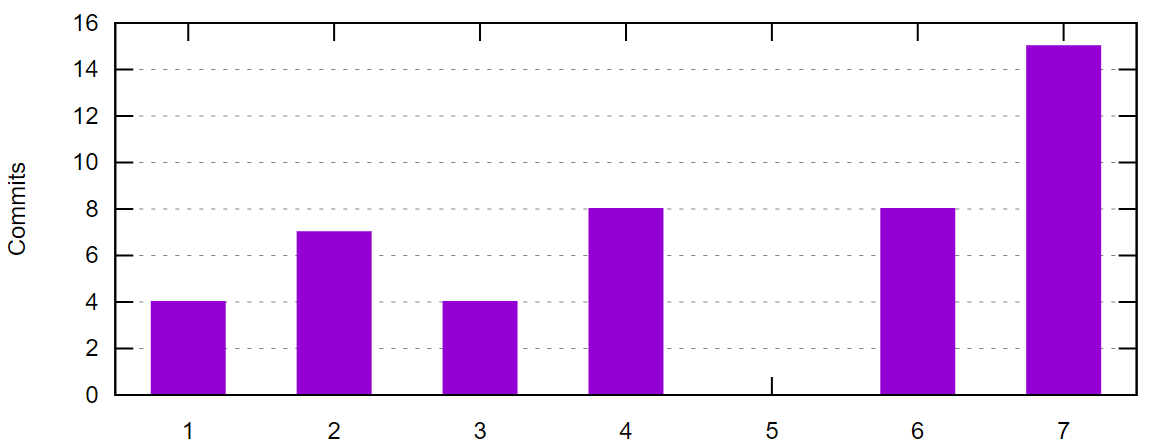
\includegraphics[width=0.95\textwidth]{../imagens/stats/days-of-week-backend.png}
	\fonte{Os autores - Criado via \gls{gitstats}}
\end{figure}